% UART core block diagram (TikZ) for the README
% Rebuild from this directory:
%   pdflatex block_diagram.tex
%   pdftoppm -png -r 200 -singlefile block_diagram.pdf block_diagram
\documentclass[border=10pt]{standalone}
\usepackage{tikz}
\usetikzlibrary{positioning,arrows.meta,fit,backgrounds,calc}
\begin{document}
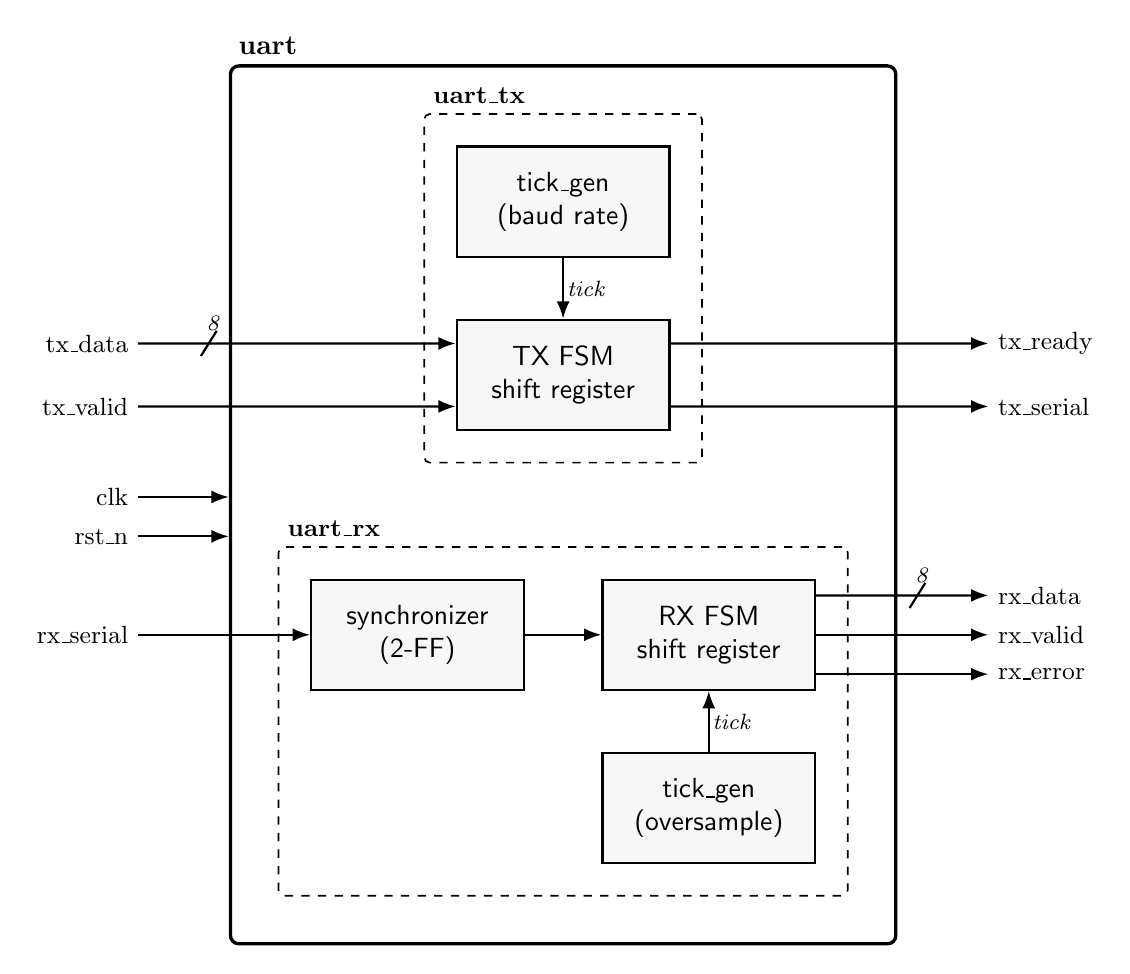
\begin{tikzpicture}[
  font=\sffamily,
  >={Latex[length=2.2mm]},
  sub/.style={draw, thick, minimum height=14mm, minimum width=27mm, align=center, fill=black!3},
  grp/.style={draw, semithick, dashed, rounded corners=2pt, inner sep=4mm},
  outer/.style={draw, very thick, rounded corners=3pt, inner sep=6mm},
  sig/.style={->, thick},
  lbl/.style={font=\small},
  slab/.style={font=\footnotesize\itshape, inner sep=1pt}
]
\newcommand{\busslash}[2]{% 
  \draw[thick] ($#1+(-1.0mm,-1.6mm)$) -- ($#1+(1.0mm,1.6mm)$);
  \node[slab, above, inner sep=1.3pt] at ($#1+(0.5mm,1.1mm)$) {#2};}

% uart_tx (centered on x=0)
\node[sub] (txfsm) at (0,0) {TX FSM\\shift register};
\node[sub] (txtick) at (0,2.2) {tick\_gen\\(baud rate)};
\draw[sig] (txtick) -- node[right,slab]{tick} (txfsm);
\begin{scope}[on background layer]
  \node[grp, fit=(txfsm)(txtick)] (tx) {};
\end{scope}
\node[anchor=south west, font=\bfseries\small] at (tx.north west) {uart\_tx};

% uart_rx (centered on x=0)
\node[sub] (sync)  at (-1.85,-3.3) {synchronizer\\(2-FF)};
\node[sub] (rxfsm) at (1.85,-3.3) {RX FSM\\shift register};
\node[sub] (rxtick) at (1.85,-5.5) {tick\_gen\\(oversample)};
\draw[sig] (sync) -- (rxfsm);
\draw[sig] (rxtick) -- node[right,slab]{tick} (rxfsm);
\begin{scope}[on background layer]
  \node[grp, fit=(sync)(rxfsm)(rxtick)] (rx) {};
\end{scope}
\node[anchor=south west, font=\bfseries\small] at (rx.north west) {uart\_rx};

% Outer uart boundary
\begin{scope}[on background layer]
  \node[outer, fit=(tx)(rx)] (uart) {};
\end{scope}
\node[anchor=south west, font=\bfseries] at (uart.north west) {uart};

% Left inputs
\def\LX{-5.4}
\node[lbl, anchor=east] (ptxd) at (\LX,0.4)  {tx\_data};
\node[lbl, anchor=east] (ptxv) at (\LX,-0.4) {tx\_valid};
\node[lbl, anchor=east] (pclk) at (\LX,-1.55) {clk};
\node[lbl, anchor=east] (prst) at (\LX,-2.05) {rst\_n};
\node[lbl, anchor=east] (prxs) at (\LX,-3.3)  {rx\_serial};
\draw[sig] (ptxd.east) -- ($(txfsm.west)+(0,4mm)$);
\busslash{($(ptxd.east)+(0.9,0)$)}{8}
\draw[sig] (ptxv.east) -- ($(txfsm.west)+(0,-4mm)$);
\draw[sig] (pclk.east) -- (pclk.east -| uart.west);
\draw[sig] (prst.east) -- (prst.east -| uart.west);
\draw[sig] (prxs.east) -- (sync.west);

% Right outputs
\def\RX{5.4}
\node[lbl, anchor=west] (ptxr) at (\RX,0.4)  {tx\_ready};
\node[lbl, anchor=west] (ptxs) at (\RX,-0.4) {tx\_serial};
\draw[sig] ($(txfsm.east)+(0,4mm)$) -- (ptxr.west);
\draw[sig] ($(txfsm.east)+(0,-4mm)$) -- (ptxs.west);
\node[lbl, anchor=west] (prxd) at (\RX,-2.8)  {rx\_data};
\node[lbl, anchor=west] (prxv) at (\RX,-3.3)  {rx\_valid};
\node[lbl, anchor=west] (prxe) at (\RX,-3.8)  {rx\_error};
\draw[sig] ($(rxfsm.east)+(0,5mm)$) -- (prxd.west);
\busslash{($(prxd.west)+(-0.9,0)$)}{8}
\draw[sig] ($(rxfsm.east)+(0,0mm)$) -- (prxv.west);
\draw[sig] ($(rxfsm.east)+(0,-5mm)$) -- (prxe.west);

\end{tikzpicture}
\end{document}
